\pdfoutput=1

\documentclass{l4proj}

%
% put any packages here
%

\begin{document}
\title{Visualisation of the Contextual Analysis and Code Generation Phases of a Compiler}
\author{David Robertson}
\date{January 1, 2000}
\maketitle

\begin{abstract}

\end{abstract}

\educationalconsent
%
%NOTE: if you include the educationalconsent (above) and your project is graded an A then
%      it may be entered in the CS Hall of Fame
%
\tableofcontents
%==============================================================================

\chapter{Introduction}
\pagenumbering{arabic}
\section{Motivation}
With increasing technological advances and furthering levels of software abstraction, some may consider compilation to be a slightly esoteric subject, in that the specific knowledge acquired can be directly applied only in a small number of highly specialized industries. Yet, remaining as a foundation of a computer science curriculum at many schools and universities is the art of compiler construction, behaviour and optimisation.

Niklaus Wirth, the creator of the Pascal programming language and renowned lecturer of compiler design states, ``\textit{knowledge about system surfaces alone is insufficient in computer science; what is needed is an understanding of contents}''. Wirth's view is one that I share, in the respect that the most successful computer scientists must have more than a superficial understanding of which approaches to follow in a given situation. They must understand how various components interact and why they behave the way they do, as this is the only way of making deeply informed technological decisions.

Compilation can often be a tricky field to teach effectively. Most compilation procedures require the construction of auxiliary data structures, commonly trees, which must be traversed in a specific manner in order to both validate the source code and create some useful output - usually an executable program. In order to illustrate this concept to students, the educator is typically restricted to creating a ``slideshow'', using an application such as Microsoft Powerpoint, in which each slide shows a distinct step of the traversal. Creating a slideshow to demonstrate these concepts is not only an onerous task on behalf of the educator, but is, more importantly, restricted to showing strictly pre-determined examples. 

\section{Background}
\subsection{ANTLR}
ANTLR (Another Tool For Language Recognition) is a popular compiler generation tool. Given a grammar written in ANTLR notation (similar to EBNF notation), ANTLR can automatically generate a lexer and a recursive-descent parser. ANTLR also generates a visitor interface, which is the foundation for implementing a contextual analyser and code generator. Please refer to appendix A for a brief outline of compilation and its constituent features, including contextual analysis and code generation.

\subsection{The Fun Programming Language}
Included in Niklaus Wirth's 1975 book {\it Algorithms + Data Structures = Programs}, is a language written entirely in Pascal named ``PL/0''. PL/0 was intended as a small educational programming language, used to teach the concepts of compiler construction. The language contains very primitive constructs and limited operations. Similarly to PL/0, ``Fun'' is a simple imperative language, developed at Glasgow University by David Watt and Simon Gay. Its purpose is to illustrate various general aspects of programming languages, including the construction of an elementary compiler. The language is provided as a supplementary aid during the delivery of the level 3 computer science course, {\it Programming Languages}, at Glasgow University.

\section{Aims}
The aim of this project is to provide a web application in which users will be able to visualise the contextual analysis and code generation phases of the Fun compiler. The visualisation will be in the form of a representation of an abstract syntax tree (AST). The mechanics of each phase will be illustrated by ``jumps'' over the AST, demonstrating the traversal that is internally taking place within the compiler. The application should:
\begin{itemize}
\item Allow a user to input and submit any syntactically valid program written in the Fun language.
\item Visualise the contextual analysis phase of a program's compilation. 
\item Visualise the code generation phase of a program's compilation.
\item Display any relevant details during the compilation, including: address/type tables, code templates, object code and explanatory messages.
\item Allow the visualisation to be ``played'' continuously or step-wise, backwards and forwards.
\end{itemize}

This application will act as a teaching tool, equally useful to educators and students alike. Students are free to use the tool outside of school/university hours in order to further their own learning. Since any arbitrary Fun program can be compiled, the restriction to educators of showing only pre-determined examples is removed. Additionally, the level of automated analysis attainable from the application is considerably greater than anything currently possible by present techniques. It will hopefully provide a better means for those looking to learn but also remove some of the struggle taken on by educators in teaching the topic.

\section{Outline}
The rest of this report is organised as follows. Chapter 2 looks at requirements gathering and elicitation. Chapter 3 discusses how the requirements were used to build an initial design of the system. Chapter 4 covers in detail the implementation of the application.

\chapter{Requirements}
\section{Methodology} 
After establishing that a product is worthwhile to build in the first place, most requirement elicitation approaches involve a repetitive cycle of expanding or reducing an initially small list of desiderata. After an initial interview with Simon Gay, the current lecturer of the {\it Programming Languages} course and proposer of this project, it was clear that whilst the project was inherently complex, the set of functional requirements was simple, well-defined and unlikely to change significantly in the future. For this reason, it was determined that extensive requirement gathering techniques, such as questionnaires or focus groups, were ultimately unnecessary; and all additional requirements were to be established through further interviews with Simon Gay.

\section{Existing Products}
Interestingly, compiler visualisation is a considerably novel area of research and development. Very few existing tools provide any illustration of the compilation process and essentially no tools exist that provide the level of analysis and step-by-step explanation of the process which this application aims to do. 

ANTLR does provide a tool for visualising the parse tree (or concrete syntax tree) generated by a grammar from an input file, as seen in figure \ref{ANTLR-parse-tree}. A parse tree contains a concrete representation of the input, retaining all information, including white-space and brackets. Conversely, an abstract syntax tree is a smaller, more concise representation of the parse tree and thus the input. An AST usually removes tokens such as white-space, brackets and other redundant details which are derivable from the structure of the tree. An illustration of what an AST might look like for the same program is shown in figure \ref{ANTLR-syntax-tree}, unfortunately, ANTLR currently provides no out-of-the-box support to build trees in this way.

Whilst this tool may serve to provide a preliminary understanding of how ANTLR forms a parse tree, we can immediately observe how large and difficult to read figure \ref{ANTLR-parse-tree} is, in comparison to figure \ref{ANTLR-syntax-tree}. There are many unnecessary tokens, such as EOFs, brackets and colons - which in most cases add nothing to the understanding of the tree. The tree also contains many branches that could easily be collapsed into a single node.

Additionally, this tool provides nothing more than a simple diagram, it gives no indication of how this tree would be traversed during compilation, nor does it give an explanation of what is happening internally at each node. 

\begin{figure}
\centering
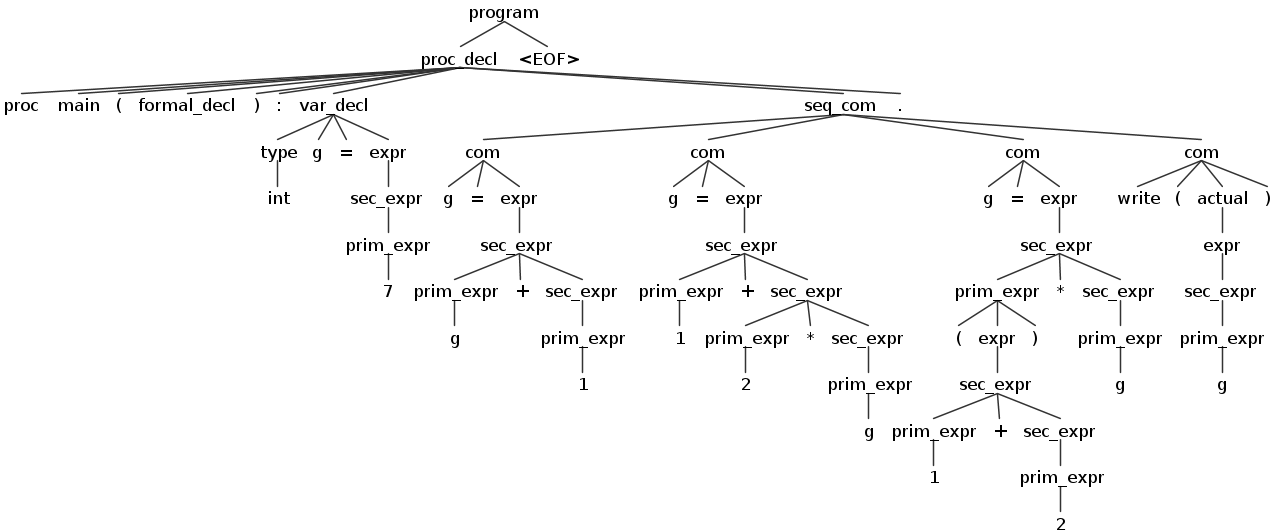
\includegraphics[height=9.2cm,width=13.2cm]{images/2-2a.png}
\caption{An ANTLR generated parse tree}
\label{ANTLR-parse-tree}
\end{figure}

\begin{figure}
\centering
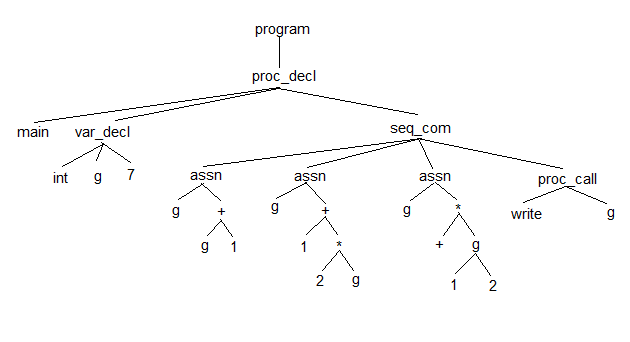
\includegraphics[height=9.2cm,width=13.2cm]{images/2-2b.png}
\caption{An AST representation of the previous tree}
\label{ANTLR-syntax-tree}
\end{figure}



%%%%%%%%%%%%%%%%
%              %
%  APPENDICES  %
%              %
%%%%%%%%%%%%%%%%
\begin{appendices}
\chapter{Compilation}
\subsection{Overview}
The term ``high-level'' language is used to refer to a programming language that provides significant levels of abstraction. These languages often allow the programmer to hide or automate several aspects of a computer system, such as memory management or garbage collection. Whilst these languages are much easier to use than their low-level counterparts, it is usually not possible to execute source code written in a high-level language directly on a computer. Examples of high-level languages are Java, C++ and Haskell.

Conversely, a ``low-level'' language provides little to no abstraction. Statements written in a low-level language often map very closely to processor instructions. Source code written in a low-level language can usually be executed directly on a computer; however, the increased complexity means it is often extremely difficult or near impossible for a human to develop software in a low-level language. Examples of low-level languages are assembly language, object code and machine code.

Compilation is the process of automatically translating high-level code into low-level code. The most common case is to convert a program whose source code is written in some programming language, into an executable program. This compilation process can usually be decomposed into three distinct phases: 
\begin{enumerate}
\item Syntactic Analysis 
\item Contextual Analysis
\item Code Generation
\end{enumerate}
Note that if any one of these phases happens to encounter an error during its execution, the entire compilation process is halted before proceeding to the next phase.

\subsection{Syntactic Analysis}
During syntactic analysis the source program is inspected to verify whether it is well-formed in accordance to the language's syntax. Syntactic analysis can itself be broken down into two further phases:
\begin{enumerate}
\item Lexing
\item Parsing
\end{enumerate}

A lexer is given a source program as input, which it breaks down into a stream of tokens. This stream is then passed to the parser which converts the token stream into an abstract syntax tree (AST) using a parsing algorithm. The parsing algorithm which is considered throughout this paper is recursive-descent parsing.

\subsection{Contextual Analysis}
Upon successful completion of syntactic analysis, the AST is traversed or ``walked'' by the contextual analyser. The contextual analyser will check whether the program represented by the AST conforms to the source language's scope and type rules. Contextual analysis can be broken down into two phases:
\begin{enumerate}
\item Scope Checking
\item Type Checking
\end{enumerate}

Scope checking ensures that every variable used in the program has been previously declared. Type checking ensures that every operation has operands of the expected type.

\subsection{Code Generation}
Upon successful completion of contextual analysis, the code generator translates the parsed program into a lower level language, such as assembly language or object code. Code generation can be broken down into two phases:
\begin{enumerate}
\item Address Allocation
\item Code Selection
\end{enumerate}

Address allocation decides the representation and address of each variable in the source program. Code selection selects and generates the object code. Upon successful completion of this final phase, the compiler will have often produced an executable program.
\end{appendices}

%%%%%%%%%%%%%%%%%%%%
%   BIBLIOGRAPHY   %
%%%%%%%%%%%%%%%%%%%%

\bibliographystyle{plain}
%\bibliography{bib}

\end{document}
